\underbar{\textbf{\large Ejercicio 1:}} Sea este diagrama:

\begin{figure}[h]
  \begin{center}
    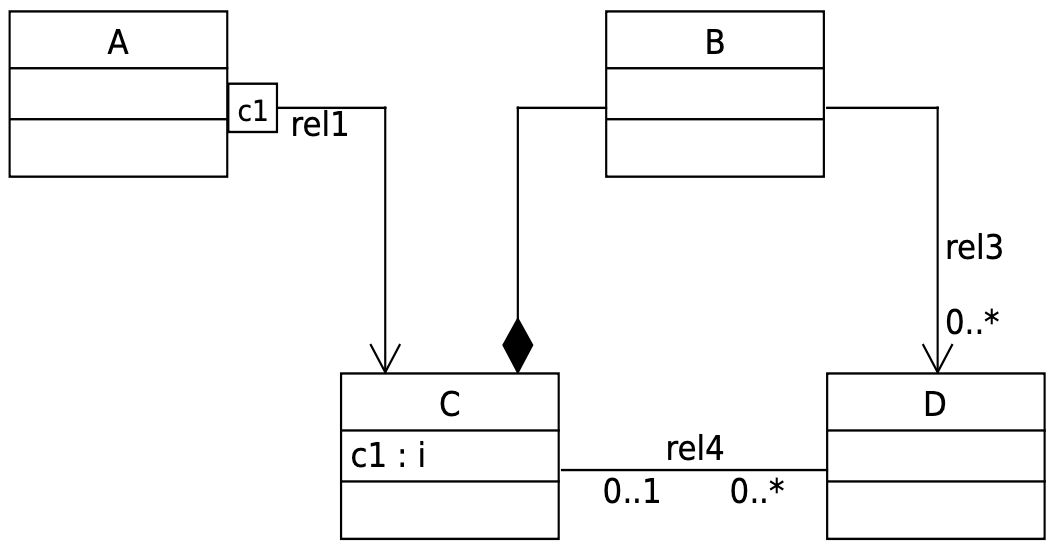
\includegraphics[width=0.6\textwidth]{assets/Junio22_1.png}
  \end{center}  
  \caption{Diagrama de clases del ejercicio}
\end{figure}

\begin{enumerate}[label = \alph*)]
  \item Escriba para cada clase los atributos estrictamente indispensables para la implementación de las relaciones en las que participa.
  
  Preguntar si hace falta implementarlas.
  \begin{minted}[breaklines]{C++}
//Como es una relacion calificada, suponemos que el tipo de dato del calificador es un entero.
class A{
  public:
    typedef std::map<size_t, C*>Calificadas;
    void rel1(C& c1)noexcept{calificadas_.insert(std::make_pair(c1.getid(),&c1));}
    const Calificadas& getCalificada()const noexcept{return calificadas_;}
  private:
    Calificadas calificadas_;
};

class C : private B{ //rel2
  public:
    C(B& b):B(b){}
    size_t getid()const noexcept{return id_;}

    //Alias de la relacion con D rel3
    typedef std::set<D*>Ds;
    void rel4(D& d)noexcept{ds_.insert(&d);}
    const DS& getD()const noexcept{return ds_;}
  private:
    size_t id_; //atributo calificador
    Ds ds_;
};




class D{
  public:
    void rel4(C& c){c_ = &c;}
    C* getC()const noexcept{return c_;}
  private:
    C* c_;
};

class B{
  public:
    //Alias del conjunto de D
    typedef std::set<D*>DS;
    void rel3(D& d)noexcept{ds.insert(&d);}
    const DS& getD()const noexcept{return ds_;}
  private:
    DS ds_;
};   
  \end{minted}
  \item Defina los constructores que estime oportunos para la clase D.
  
  La clase D va a tener solamente un constructor por defecto, debido a que no recibe ningún parámetro procedente de otras clases relacionadas, ya que un objeto de la clase C puede estar o no instaciado con uno de la clase D (multiplicidad 0..1) y la relación con la clase B es unidireccional, por tanto, no recibe el objeto o puntero de la clase B.

  \item Suponga que se añade un atributo de enlace de tipo X a rel3 ¿cómo cambiariarían los miembros?
   
  Sabemos que tenemos una relación de asociación unidireccional 1 - muchos entre las clases B y D (rel3), si nos ceñimos a la teoría sabemos que el atributo de enlace se guarda en la clase que tiene la multiplicidad muchos (D), por tanto no cambiaría nada ya que la clase B seguiría recibiendo un conjunto (set) de punteros de tipo D, y en D se guardaría dicho atributo de enlace en su parte privada.
\end{enumerate}

\newpage
\underbar{\textbf{\large Ejercicio 2:}} Implemente la rel4 del ejercicio anterior mediante una clase de asociación. Para ello:

\begin{enumerate}[label = \alph*)]
  \item Defina la clase con los atributos que estime oportunos declarando dos métodos \texttt{asocia()} y otros dos llamados \texttt{asociados()}, una pareja para cada sentido de la relación.
  \item Defina las funciones miembro \texttt{asocia()} de tal forma que ambas permitan crear/modificar el doble enlace entre un objeto de C y otro de D. Si D ya está asociado a un C, se desvinculará del mismo y se enlazará al nuevo.
  \item Defina las dos funciones miembro \texttt{asociados()}.
\end{enumerate}
\begin{minted}[breaklines]{C++}
class CD{
public:
  //Alias del conjunto de punteros de tipo D
  typedef std:: set<D*> Ds;
  
  //Alias de las relaciones
  typedef std::map<C*,Ds> CDs;
  typedef std::map<D*,C*> DC;

  void asocia(C& c, D& d)noexcept{
    //Si D está asociado con otro C, se desvincula y se asocia el que le pasamos por parámetro
    auto i = inversa_.find(&d);
    if(i!=inversa_.end()){ //D está asociado con un C
      directa_[i->second].erase(&d);//eliminamos el antiguo D.
    }
    inversa_[&d]=&c;
    directa_[&c].insert(&d);
  }
  void asocia(D& d,C& c)noexcept{asocia(c,d);}

  Ds asociados(C& c)const noexcept{
    auto i = directa_.find(&c);
    if(i != directa_.end()) return i->second;
    else{
      //Devolvemos un conjunto vacio
      CD::Ds vacio;
      return vacio;
    }
  }

  C* asociados(D& d)const noexcept{
    auto i = inversa_.find(&d);
    if(i!=inversa_.end()) return i->second;
    return nullptr;
  }
private:
  CDs directa_;
  DC inversa_;
};
\end{minted}
\underbar{\textbf{\large Ejercicio 3 :}} Dadas las siguientes definiciones de clases:
\begin{center}
  \begin{verbatim}
________________________________________________________________________________
struct X{
  X(char c) : c(c) { cout << "Ctor. de X" << endl; } char c;
};

struct A{ 
  A(X x);
  void f() { cout << "Método f() de A" << endl; } ~A() { cout << "Dtor. de A" << endl; }
  X x;
};
struct B{
  B(X x);
  void f() { cout << "Método f() de B" << endl; } ~B() { cout << "Dtor. de B" << endl; }
  X x;
};
________________________________________________________________________________
  \end{verbatim}
\end{center}
\begin{enumerate}[label = \alph*)]
  \item Escriba las definiciones de los constructores de A y B de forma que impriman el texto del constructor de A y el constructor de B respectivamente.
  
\begin{minted}[breaklines]{C++}
struct A{
  A(X x): x(x){}
  void f() { cout << "Método f() de A" << endl; } ~A() { cout << "Dtor. de A" << endl; }
  X x;
};

struct B{
  B(X x):x(x){}
  void f() { cout << "Método f() de B" << endl; } ~B() { cout << "Dtor. de B" << endl; }
  X x;
};
\end{minted}
\end{enumerate}